\documentclass[12pt]{article}
\usepackage[utf8]{inputenc}

\usepackage{lmodern}

\usepackage{enumitem}
\usepackage[margin=2cm]{geometry}

\usepackage{amsmath, amsfonts, amssymb}
\usepackage{graphicx}
%\usepackage{subfigure}
\usepackage{tikz}
\usepackage{pgfplots}
\usepackage{multicol}

\usepackage{comment}
\usepackage{url}
\usepackage{calc}
\usepackage{subcaption}
\usepackage[indent=0pt]{parskip}
\usepackage{animate}

\usepackage{array}
\usepackage{blkarray,booktabs, bigstrut}
\usepackage{bigints}

\pgfplotsset{compat=1.16}

% MATH commands
\newcommand{\ga}{\left\langle}
\newcommand{\da}{\right\rangle}
\newcommand{\oa}{\left\lbrace}
\newcommand{\fa}{\right\rbrace}
\newcommand{\oc}{\left[}
\newcommand{\fc}{\right]}
\newcommand{\op}{\left(}
\newcommand{\fp}{\right)}

\newcommand{\bi}{\mathbf{i}}
\newcommand{\bj}{\mathbf{j}}
\newcommand{\bk}{\mathbf{k}}
\newcommand{\bF}{\mathbf{F}}

\newcommand{\mR}{\mathbb{R}}

\newcommand{\ra}{\rightarrow}
\newcommand{\Ra}{\Rightarrow}

\newcommand{\sech}{\mathrm{sech}\,}
\newcommand{\csch}{\mathrm{csch}\,}
\newcommand{\curl}{\mathrm{curl}\,}
\newcommand{\dive}{\mathrm{div}\,}

\newcommand{\ve}{\varepsilon}
\newcommand{\spc}{\vspace*{0.5cm}}

\DeclareMathOperator{\Ran}{Ran}
\DeclareMathOperator{\Dom}{Dom}

\newcommand{\exo}[1]{\noindent\textcolor{red}{\fbox{\textbf{Problem {#1}}}\hrulefill}\\\\ }
\newcommand{\qu}[4]{\noindent\textcolor{#4}{\fbox{\textbf{Section {#1} | Problem {#2}}} \hrulefill{{\fbox{\textbf{{#3} Points}}}}\\}}

\newcommand{\semester}{Fall 2023}

\newcommand{\CVup}{%
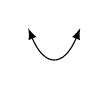
\begin{tikzpicture}
\draw[black, <->, >=latex] (-0.33, 0.5) .. controls (-0.125, 0) and (0.125, 0) .. (0.33, 0.5);
\end{tikzpicture}}

\newcommand{\CVupInc}{%
\begin{tikzpicture}
\draw[black, ->, >=latex] (0,0) .. controls (0.2, 0) and (0.4, 0.2) .. (0.5, 0.5);
\end{tikzpicture}}

\newcommand{\CVupDec}{%
\begin{tikzpicture}[rotate=270]
\draw[black, ->, >=latex] (0,0) .. controls (0.2, 0) and (0.4, 0.2) .. (0.5, 0.5);
\end{tikzpicture}}

\newcommand{\CVdown}{%
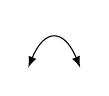
\begin{tikzpicture}
\draw[black, <->, >=latex] (-0.33, -0.5) .. controls (-0.125, 0) and (0.125, 0) .. (0.33, -0.5);
\end{tikzpicture}}

\newcommand{\CVdownInc}{%
\begin{tikzpicture}
\draw[black, ->, >=latex] (-0.5, -0.5) .. controls (-0.5, -0.3) and (-0.5, -0.1) .. (0,0);
\end{tikzpicture}}

\newcommand{\CVdownDec}{%
\begin{tikzpicture}[rotate=-90]
\draw[black, ->, >=latex] (-0.5, -0.5) .. controls (-0.5, -0.3) and (-0.5, -0.1) .. (0,0);
\end{tikzpicture}}

\begin{document}
	\noindent \hrulefill \\
	MATH-244 \semester \hfill Practice Problems Solutions\\
	Section 16.1 \hfill Pierre-Olivier Paris{\'e} \\\vspace*{-1cm}
	
	\noindent\hrulefill
	
	\spc	

	\exo{16}
	When $z = 0$, each $(x, y, 0)$ is mapped to $\bi + 2 \bj$. So in the $xy$-plane, we should have the same vectors. This is exactly the plot I.

	\spc

	\exo{18}
	When $x$, $y$, and $z$ are small, the vector $x\bi + y \bj + z \bk$ has a small length. If $x \neq 0$, $y = \neq 0$, and $z \neq 0$, then the vector $x\bi + y \bj + z \bk$ is pointing in the opposite direction of the origin (like a vector emanating from the origin, starting at the point $(x, y, z)$). Also, we see that if $x = y = z = 0$, then we obtain the zero vector. The only plot that has the zero vector is the plot II.
	
	\spc
	
	\exo{26}
	We have
		\begin{align*}
		f_x (x, y) = x \quad \text{ and } \quad f_y (x, y) = -y .
		\end{align*}
	So the gradient vector field is $\nabla f = \bF (x, y) = x\bi - y \bj$. The picture below shows a plot of the vector field.
		\begin{figure}[h]
		\centering
		\includegraphics[scale=0.4]{vectorFieldGradient.png}
		\end{figure}

	\spc

	\exo{30}
	The function is $f(x) = x^2 + xy$. So its gradient is $\vec{\nabla} f (x, y) = (2x + y) \vec{i} + x \vec{j}$. The $x$-coordinate of the vector field is zero if $y = -2x$. In this case, the vector field looks like
		\begin{align*}
		\vec{\nabla}f (x, y) = -(y/2) \vec{j} .
		\end{align*}
	Also, when $y > -2x$, then the $x$ coordinate of the vector field is positive and all the vectors in the vector field must point to the east (to the right, in the same direction to the positive $x$-axis). When $y < -2x$, then the $x$ coordinate of the vector field is negative and all the vectors in the vector field must point to the west (to the left, in the opposite direction to the positive $x$-axis).
	
	So the corresponding representation is IV.

	\spc
	
	\exo{34}
	The vector at $(x, y) = (1, 3)$ is $\vec{F}(1, 3) = \left\langle 1, -1 \right\rangle$. So, the new position of the particle would be 	
	\begin{align*}
	\left\langle x_1 , y_1 \right\rangle = (1, 3) + \Delta t \vec{F} (1, 3) = \left\langle 1, 2 \right\rangle + 0.05 \left\langle 1 , -1 \right\rangle = \left\langle 1.05 , 1.95 \right\rangle .
	\end{align*}



\end{document}